\documentclass{article}
\usepackage[margin=1in]{geometry}
\usepackage{graphicx}
\usepackage{amsmath}
\usepackage{enumitem}
\usepackage{hyperref}

\title{CSCI/ROBO 7000/4830: DEEP REINFORCEMENT LEARNING AND ROBOTICS \\ FALL 2025 \\ HOMEWORK \#2: MODEL-FREE CONTROL AND CREDIT ASSIGNMENT}
\author{Steve Gillet}
\date{\today}

\begin{document}

\maketitle

\section{Introduction}

This assignment dives into the core of model-free reinforcement learning. In the last assignment, you worked with a known model of the world (a deterministic MDP). Now, you'll implement agents that learn optimal policies directly from experience, without any prior knowledge of the environment's dynamics or reward functions.

You will implement and compare two fundamental Temporal Difference (TD) control algorithms, SARSA and Q-Learning, to understand the critical difference between on-policy and off-policy learning. Then, you will implement SARSA($\lambda$) to explore how eligibility traces provide an elegant solution to the credit assignment problem in environments with delayed rewards.

\textbf{A Note on Academic Integrity:} The reasoning questions in this assignment are designed to test your unique understanding of the concepts and your specific results. You must be able to connect the theory from the lectures directly to the behavior you observe from your own code.

\textbf{Note \#2:} You are expected to submit both a working code AND collect your answers in a PDF file. Failure to do so will result in points being cut.

\section{PART 1: ON-POLICY VS. OFF-POLICY CONTROL IN "CLIFF WALKING" [40 POINTS]}

In this part, we will use the classic "Cliff Walking" environment to see how an agent's learning strategy is directly influenced by the choice between an on-policy and an off-policy algorithm.

\subsection{THE ENVIRONMENT: CLIFFWALKING-V1}

You will use the CliffWalking-v1 environment from the gymnasium library. You do not need to implement the environment yourself. More info here \href{[LINK]}{[LINK]}.

\begin{itemize}
    \item Goal: Navigate from a start state (S) to a goal state (G) on a 4x12 grid with the goal located at [3, 11].
    \item The Cliff: The bottom row of the grid is a cliff. Stepping on a cliff tile results in a large negative reward and sends the agent back to the start.
    \item Rewards:
    \begin{itemize}
        \item R = -1 for every step in a non-cliff, non-goal state.
        \item R = -100 for stepping on a cliff tile.
        \item The episode terminates upon reaching the goal (G).
    \end{itemize}
\end{itemize}

\subsection{1.1. IMPLEMENTATION: SARSA AND Q-LEARNING AGENTS [20/40 POINTS]}

Your task is to implement two agents. You should use NumPy for your Q-tables and mathematical operations.

\begin{enumerate}[label=\Alph*.]
    \item SarsaAgent: An on-policy TD control agent. It implements the update method using the SARSA update rule (see slides).
    \item QLearningAgent: An off-policy TD control agent. It implements the update method using the Q-Learning (SARSAMAX) update rule (see slides).
\end{enumerate}

Both agents should use an $\epsilon$-greedy policy for action selection.

% Your code implementation goes here (but submit separately)

\subsection{1.2. ANALYSIS \& REASONING [20/40 POINTS]}

Run both agents in the environment for 500 episodes and use your results to answer the following questions.

\begin{itemize}
    \item After training, visualize the final policy for both the SARSA and Q-Learning agents by drawing arrows on a grid to show the best action from each state.
    
    SARSA:

    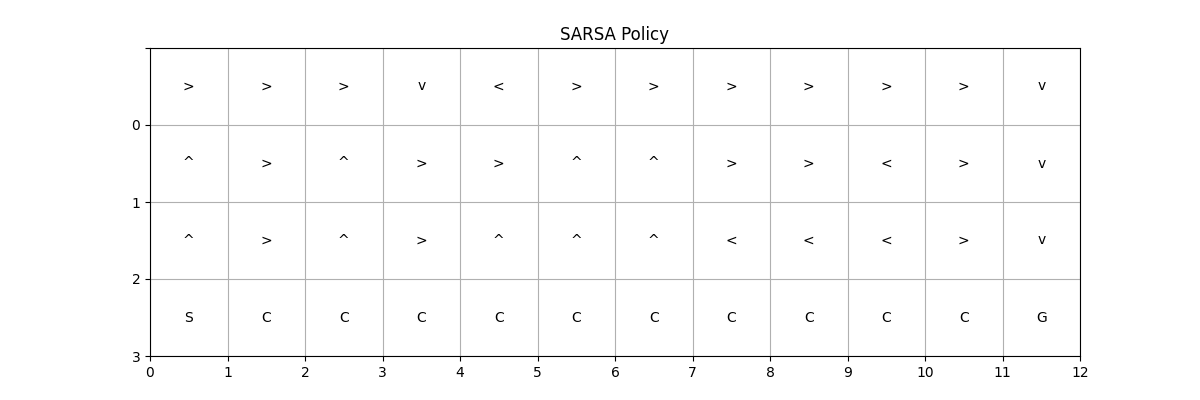
\includegraphics[width=0.9\textwidth]{sarsaGrid.png}

    SARSAMAX:

    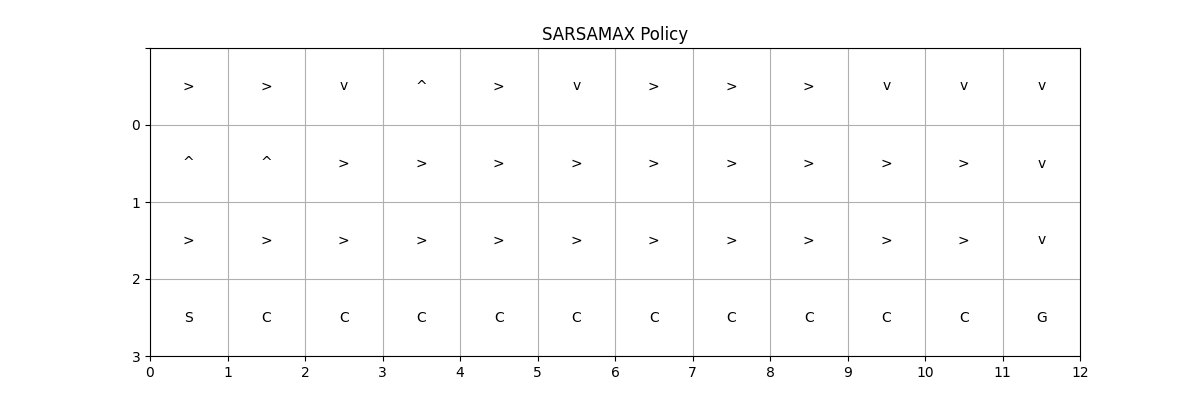
\includegraphics[width=0.9\textwidth]{sarsaMaxGrid.png}
    
    \item Describe the difference between the two policies. Which one finds the "optimal" (shortest) path? Which one finds the "safer" path? Explain why this difference emerges by referencing the specific components of their respective update equations.
    
    SARSA is updating its $\epsilon$-greedy exploration policy while it is executing it, sometimes the next state that it updates is a random step that takes it off the cliff causing a large negative penalty and pushing the policy away from the cliff.
    SARSAMAX is executing the $\epsilon$-greedy exploration policy but only updating the greedy policy, so while it might randomly step off the cliff it is still updating the value based on the optimal action.
    
    \item Plot the "Sum of Rewards per Episode" for both agents on the same graph (with episodes on the x-axis). Which agent achieves better overall performance (higher cumulative reward) during the learning process? Explain this result in the context of their different policies.
    
    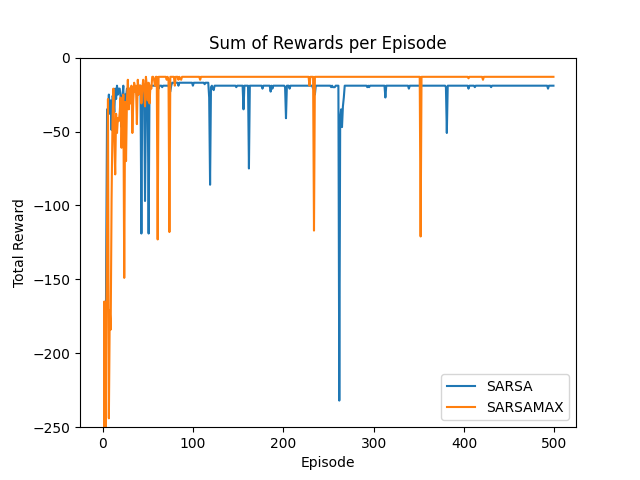
\includegraphics[width=0.9\textwidth]{rewardsComparison.png}
    
    You can see the SARSAMAX getting pretty consistently higher rewards which makes sense given that you are acting more greedily.
    There is a higher value on the greedy states and actions so the agent is more likely to go that way and the rewards are going to be higher because that behavior is going to result in shorter paths.

1`247'\end{itemize}

\section{PART 2: TD, MC, AND BOOTSTRAPPING [20 POINTS]}

This part is a conceptual check to ensure you understand the mechanics of TD learning compared to Monte Carlo methods.

Hint: No coding is required to answer the below. However, now that you do have the code working from Part 1, you might find it useful to create some code to check your answers!

\subsection{THE "ONE-EPISODE TEST"}

Imagine you run your SARSA agent on "Cliff Walking" for only one single episode. By chance, the agent successfully navigates the long, safe path far from the cliff and reaches the goal.

\begin{itemize}
    \item If you were using an Every-Visit Monte Carlo Control algorithm, which state-action pairs' Q-values would be updated after this single episode is complete? Briefly describe how the return would be calculated.
    
    All of the state-action pairs that were visited would be updated and the return would be the total discounted reward from that timestep forward.
    
    \item Now, describe which Q-values would have been updated using the SARSA (TD) algorithm you implemented. How does the timing and scope of the updates differ from the MC approach?
    
    The same Q-values would be updated but the values would be updated immediately instead of having to wait till the end of the episode and they would be updated just using the rewards for the current state and the next state instead of the entire return.
    
    \item Explain why this difference occurs, using the terms bootstrapping and TD target in your explanation. Your answer should clarify why TD can learn online from incomplete sequences while MC must wait for the final outcome.
    
    TD target is that estimated return that is taken from the current and next state-action pair.
    Bootstrapping is process of making an estimate with an estimate, when you estimate the current return using the reward and the estimate based off of the next reward you are bootsrapping.
    This is the reason why TD can learn online, it uses these techniques to update the value of a state-action pair based on an estimate instead of waiting to finish the episode and calculating the actual return.
     
\end{itemize}

\section{PART 3: CREDIT ASSIGNMENT WITH SARSA($\lambda$) [40 POINTS]}

In this part, you'll investigate how eligibility traces solve the credit assignment problem in an environment with sparse, delayed rewards.

\subsection{THE ENVIRONMENT: THE "DELAYED REWARD MAZE"}

You are be provided with a simple 5x5 maze environment.

\begin{itemize}
    \item Goal: Navigate from a start state (S) to a goal state (G).
    \item Rewards:
    \begin{itemize}
        \item R = +10 for entering the Goal state. The episode then terminates.
        \item R = 0 for all other transitions.
    \end{itemize}
\end{itemize}

This setup is challenging because the reward signal only appears at the very end of a successful episode, making it difficult for a one-step method to assign credit to the early actions that were part of the optimal path.

\subsection{3.1. IMPLEMENTATION: SARSALAMBDAAGENT [20/40 POINTS]}

Implement a new agent, SarsaLambdaAgent, that uses backward-view SARSA($\lambda$) with accumulating eligibility traces.

\begin{itemize}
    \item Initialization: Your agent will need a Q-table and an Eligibility Trace table, $e(S, A)$, of the same dimensions, both initialized to zeros.
    \item Update Logic: At each step, you must perform the following:
    \begin{itemize}
        \item Calculate the TD error $\delta_t$ (see slides)
        \item Increment the eligibility trace for the current state-action pair
        \item Loop through all state-action pairs to update their Q-values and decay their traces
    \end{itemize}
    \item Episode Reset: Remember to reset the eligibility trace table to all zeros at the start of each new episode.
\end{itemize}

Hint: Remember that the agent explores randomly. You should expect really long episodes, especially in the beginning! 20M steps are normal.

% Your code implementation goes here (but submit separately)

\subsection{3.2. VISUALIZATION AND ANALYSIS [20/40 POINTS]}

\begin{enumerate}
    \item Run your agent for a single successful episode. After the final step (upon reaching the goal), create a heatmap of the table. This heatmap shows the "credit" trail left by the agent. Generate one heatmap for each of the following values:
    \begin{enumerate}[label=\alph*.]
        \item $\lambda = 0.2$ (Rapid decay)
        \item $\lambda = 0.7$ (Moderate decay)
        \item $\lambda = 0.95$ (Slow decay)
    \end{enumerate}
    
    % Insert your heatmaps here (e.g., \includegraphics{} for each)
    
    \item Describe how the "trail" of eligibility changes as you increase $\lambda$. Why does the credit propagate further back in time for higher values?
    
    % Your answer here
    
    \item What does the SARSA($\lambda$) algorithm become when $\lambda = 0$? Now, considering the offline updates after a full episode, what algorithm is SARSA(1) equivalent to?
    
    % Your answer here
    
    \item Based on this experiment, provide a concluding explanation for why eligibility traces are so effective for problems with delayed rewards.
    
    % Your answer here
\end{enumerate}

\section{INSTALLATION STEPS}

This project requires Python 3.8 or newer. The necessary libraries are Gymnasium for the environment, NumPy for handling the Q-tables, and Matplotlib for plotting the results.

You can install all of them with a single command using pip, Python's package installer. Open your terminal or command prompt and run the following command:

\texttt{pip install gymnasium numpy matplotlib}

\texttt{pip install time gymnasium[toy-text]}

Note: the second command is optional. You’ll need it if you’d like to visualize the agent playing in the environment!

That's it! After the installation completes, your environment will have everything needed to run the homework code.

\end{document}